\chapter{Keyboard and Mouse}

The \jr\ provides a single PS/2 port for use with either a keyboard or a mouse. This port is accessed through five registers, which provide very simple access to a PS/2 device. The \jr\ does not have a full PS/2 controller, but instead provides mostly raw access to the data stream. It does make some attempt to translate set 2 scan codes to ASCII character code, although raw scan codes may be read instead. See table \ref{tab:ps2_reg} for details.

\begin{table}[ht]
    \begin{center}
        \begin{tabular}{|c|c|c|c|c|c|c|c|c|c|c|} \hline
            Address & R/W & Name & 7 & 6 & 5 & 4 & 3 & 2 & 1 & 0 \\\hline\hline
            \verb+0xD640+ & R/W & PS2\_CTRL & \multicolumn{2}{|c|}{---} & MCLR & KCLR & M\_WR & --- & K\_WR & --- \\\hline
            \verb+0xD641+ & R/W & PS2\_OUT & \multicolumn{8}{|l|}{Data to send to keyboard} \\ \hline
            \verb+0xD642+ & R & KBD\_IN & \multicolumn{8}{|l|}{Data from the keyboard input FIFO} \\ \hline
            \verb+0xD643+ & R & MS\_IN & \multicolumn{8}{|l|}{Data from the mouse input FIFO} \\ \hline
            \verb+0xD644+ & R & PS2\_STAT & K\_AK & K\_NK & M\_AK & M\_NK & \multicolumn{2}{|c|}{---} & MEMP & KEMP \\ \hline
        \end{tabular}
    \end{center}
    \caption{PS/2 Port Registers}
    \label{tab:ps2_reg}
\end{table}

\begin{description}
    \item[K\_WR] set to 1 then 0 to send a byte written on PS2\_OUT to the keyboard
    \item[M\_WR] set to 1 then 0 to send a byte written on PS2\_OUT to the mouse
    \item[KCLR] set to 1 then 0 to clear the keyboard input FIFO queue.
    \item[MCLR] set to 1 then 0 to clear the mouse input FIFO queue. 
    \item[K\_AK] when 1, the code sent to the keyboard has been acknowledged
    \item[K\_NK] when 1, the code sent to the keyboard has resulted in an error
    \item[M\_AK] when 1, the code sent to the keyboard has been acknowledged
    \item[M\_NK] when 1, the code sent to the keyboard has resulted in an error
    \item[KEMP] when 1, the keyboard input FIFO is empty
    \item[MEMP] when 1, the mouse input FIFO is empty 
\end{description}

\section*{Mouse Support}

The \jr\ provides special support for a PS/2 mouse, including support for a hardware mouse pointer.

This is currently done with magic, the details of which will be made apparent when the stars are in proper alignment.

\subsection*{Mouse Pointer}

The \jr\ provides for a grayscale hardware mouse pointer. The pointer is a $16 \times 16$ grayscale image of 256 levels. Each pixel of the image is a single byte. The bitmap data is stored in the address range 0xCC00--0xCFFF.

The position of the mouse pointer is controlled in one of two ways. In the default approach (MODE = 0), the system software will monitor mouse movements, determine the mouse position programmatically, and set the TinyVicky mouse position registers directly. In the legacy approach (MODE = 1), the system software will receive the three byte PS/2 mouse data packet and set the TinyVicky mouse PS2\_BYTE registers. In this legacy mode, TinyVicky will interpret the mouse packets and track the mouse position for the system. This approach is less work for the system software, but is less flexible.

\begin{table}[ht]
    \begin{center}
        \begin{tabular}{|c|c|c|c|c|c|c|c|c|c|} \hline
            Address & R/W & 7 & 6 & 5 & 4 & 3 & 2 & 1 & 0 \\\hline\hline
            \verb+0xD6E0+ & W & \multicolumn{6}{|c|}{---} & MODE & EN \\\hline
            \verb+0xD6E2+ & RW & X7 & X6 & X5 & X4 & X3 & X2 & X1 & X0 \\\hline
            \verb+0xD6E3+ & RW & X15 & X14 & X13 & X12 & X11 & X10 & X9 & X8 \\\hline
            \verb+0xD6E4+ & RW & Y7 & Y6 & Y5 & Y4 & Y3 & Y2 & Y1 & Y0 \\\hline
            \verb+0xD6E5+ & RW & Y15 & Y14 & Y13 & Y12 & Y11 & Y10 & Y9 & Y8 \\\hline
            \verb+0xD6E6+ & W & \multicolumn{8}{|c|}{PS2\_BYTE\_0} \\\hline
            \verb+0xD6E7+ & W & \multicolumn{8}{|c|}{PS2\_BYTE\_1} \\\hline
            \verb+0xD6E8+ & W & \multicolumn{8}{|c|}{PS2\_BYTE\_2} \\\hline
        \end{tabular}
    \end{center}
    \caption{Mouse Pointer Registers}
    \label{tab:mouse_reg}
\end{table}

\begin{description}
    \item[EN] if set (1), the mouse pointer is displayed. If clear (0), the mouse pointer is not displayed
    \item[MODE] if clear (0), the mouse position is specified by setting the X and Y registers. If set (1), the program must pass along the 3 byte PS/2 mouse packet to the packet registers (this is a legacy mode).
    \item[X] this is the X coordinate of the mouse and both readable and writable if MODE is clear (0)
    \item[Y] this is the Y coordinate of the mouse and both readable and writable if MODE is clear (0)
    \item[PS2\_BYTE\_0] the first byte of the PS/2 mouse message packet. Only used if MODE is set (1).
    \item[PS2\_BYTE\_1] the second byte of the PS/2 mouse message packet. Only used if MODE is set (1).
    \item[PS2\_BYTE\_2] the third byte of the PS/2 mouse message packet. Only used if MODE is set (1).
\end{description}

\section*{\fk\ Keyboard}
\label{sec_f256k_kbd}

\begin{note}
    this section pertains to the \fk\ only and is not relevant to the \jr.
\end{note}

The \fk\ includes a second WDC65C22 VIA chip at 0xDB00 on I/O page 0 (see page \pageref{chap_via} for details on the VIAs) which manages the keyboard input from the \fk's built-in keyboard. The F256K's keyboard is a matrix keyboard. Except for the RESTORE key, all keys on the keyboard are arranged in a matrix with the columns assigned to VIA1's PB pins and the rows assigned to VIA1's PA pins. VIA0's PB7 pin is also used for a column. See figure~\ref{fig:f256k_matrix}.

\begin{figure}[ht]
    \begin{center}
        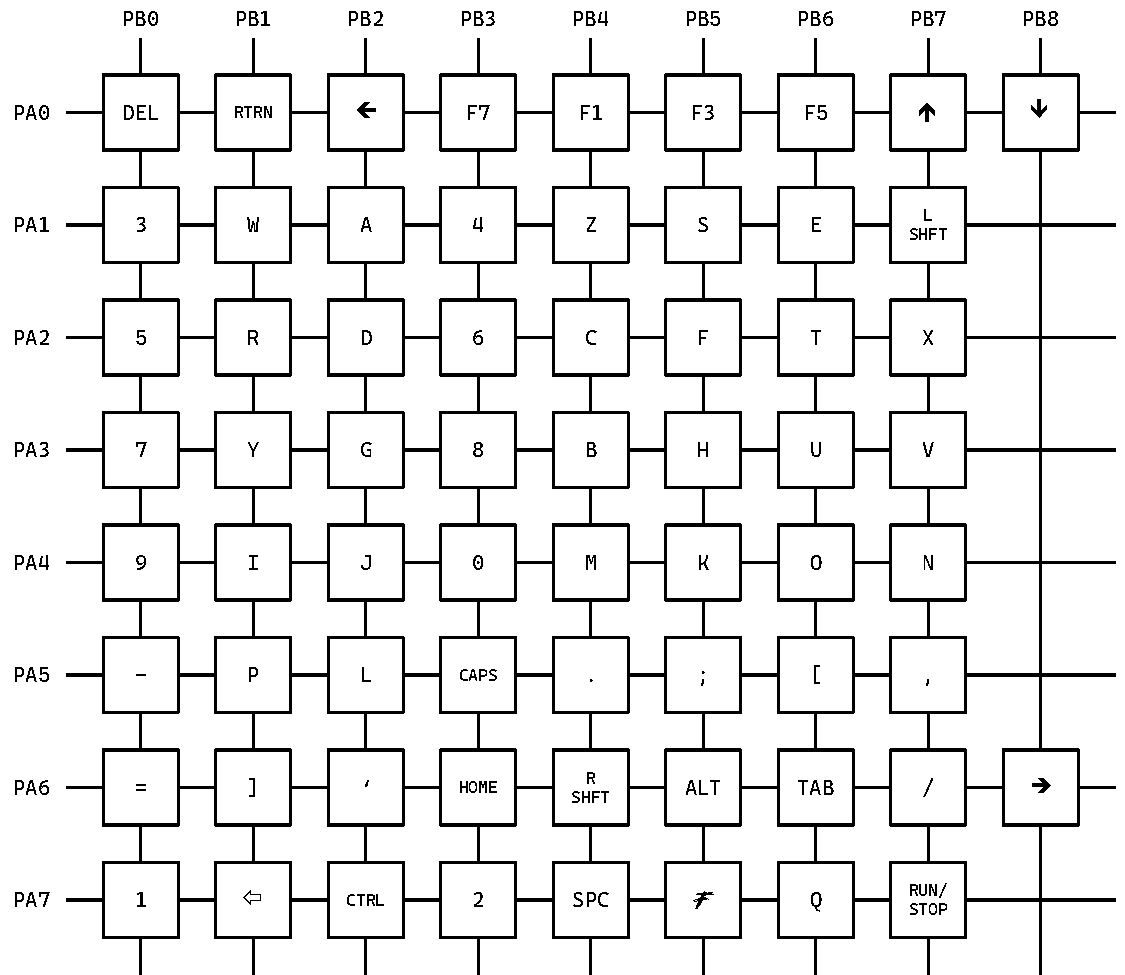
\includegraphics[scale=0.65]{images/f256k_matrix.pdf}
    \end{center}
    \caption{\fk\ Keyboard Matrix}
    \label{fig:f256k_matrix}
\end{figure}

The \fk\ keyboard includes three indicator RGB LEDs that can be set under program control. The three LEDs are for power, media access (SD and IEC), and the shift lock indicator. Each LED has three single byte registers to set the red, green, and blue component intensities for the desired colors. See table~\ref{tab:f256k_kbd_leds}.

\begin{table}[ht]
    \begin{center}
        \begin{tabular}{|c|c|c|c|} \hline
            Indicator & Address & R/W & Color \\\hline\hline
            \multirow{3}{*}{Power} & 0xD6A7 & W & Blue \\\cline{2-4}
                                   & 0xD6A8 & W & Green \\\cline{2-4}
                                   & 0xD6A9 & W & Red \\\hline

            \multirow{3}{*}{Media} & 0xD6AA & W & Blue \\\cline{2-4}
                                   & 0xD6AB & W & Green \\\cline{2-4}
                                   & 0xD6AC & W & Red \\\hline

            \multirow{3}{*}{Shift} & 0xD6AD & W & Blue \\\cline{2-4}
                                   & 0xD6AE & W & Green \\\cline{2-4}
                                   & 0xD6AF & W & Red \\\hline
        \end{tabular}
    \end{center}
    \caption{\fk\ Keyboard LEDs}
    \label{tab:f256k_kbd_leds}
\end{table}